\par
% In this chapter, we will describe the different methodologies used for different solutions. Since we have both non-machine learning and machine learning-based solutions so we have tried different approaches to solve the problem. Also, within the machine learning based solutions, we have used different approaches like in one solution we took the help of transfer learning models while in other solution we developed the model by ourselves. The reason why we opt-in for different solutions is to understand the nature of the problem and at the same time have the alternates to use one of them. The problem with machine learning based solutions is that we do not have full control of the system and cannot fix the problem instantly. A considerable amount of time has to spend to figure out the problem and to fix it. That is why some organizations are still reluctant to try this approach. In the further sections, we will discuss the methodologies for each solution one by one and will explain them in detail. 
% \section{Methodology used for Solution I}
% \par
% This solution is not using any machine learning techniques but rather using a custom algorithm to predict the document type. Although in this solution, we are using the document files in the form of pdfs for the solution, but this system will be able to classify the document type in the form of pdf or image both. This solution is predicting the document type by analyzing the content of the document and perhaps rely on the textual information from documents. To do this, we are using some third-party libraries in this solution for various purposes. For Instance, in this solution, we first have to generate a dictionary of vocabularies that will contain all the meaningful and relevant keywords for each document type. So, to develop this dictionary, we are extracting the content from all the pdfs and applying a method to pick the relevant words from them. This pdf extraction is done by a third-party library called \q{tika} \cite{tika} which is responsible for text extraction from pdf. Also, during the classification of the document, in case if the document is image then we have to extract the text from the image. For text extraction from the image, we are using python's library \q{pytesseract} \cite{pytesseract}. As far as the algorithm is concerned, it is a custom implementation that checks the score of each document type by analyzing its content and return the type with the highest frequency. We will study this algorithm in detail in Chapter \ref{chap:5}.
% \section{Methodology used for Solution II}
% In this solution, we leveraged machine learning power to provide a solution for document classification. This solution is also based on the information of textual content from the documents. Here, a neural network model is developed by the help of Keras library specifically named \q{Sequential} API \cite{seq_api}. To train this model, we used our generated dataset in the form of pdf. Since this solution is also based on textual information so we extracted the data from pdfs by using the previously mentioned third party libraries and stored the content in an array. For model training, we are passing the input in the form of a vector array. To convert the text inputs into vectors, we are using the \q{Bag of Words (BoW)} model \cite{bow} approach with the help of Keras library's class \q{Tokenizer} \cite{tokenizer}. We will explain both the Bag of words model and the Neural network model in the further sections.
% \subsection{Bag of Words (BoW)}
% In general, a bag of word model is a data modeling technique by extracting features from the text. It is normally used in the pre-processing of textual data which we also use in machine learning projects. Whenever we work on a machine learning project where we have to train the model with textual data, we cannot directly pass this data to our model as a training source because machines do not understand raw text and here we need to pre-process it and convert it into a form which can be understood by our model. There a lot of unstructured data nowadays and text is one of the foremost sources of it. We have a lot of tools that we can use to break this text down and quantify it so that we can use it in modeling. The bag of word model is one of the ways to mitigate this problem. This is a kind of core of the field called "Natural Language Processing". This quantification of text into features that we can use for our statistical models and ideally for our training models in machine learning. So, in the bag of words, first, we take our corpus (full set of documents) that we want to quantify, and we tokenize everything which means we break out every single individual word in the corpus so that we can have a look at them all together. After that, we filter out the stop words from the words list to maintain the relevancy. Stop words are the words (like a, an, the, and, or, we, etc.) that appear very frequently in the language or sentence but do not have a lot of informational content. So, we can cut all of these out without losing the important information density from our corpus. After removing the stop words, we take the remaining meaningful tokens and apply stemming or lemmatization for generalization. Basically, both of these try to get at the root word for every single word in a corpus.  Stemming is a process of reducing the word to its stem. Lemmatization is a process that uses a fork vocabulary and analyzes all the words in the corpus to get the actual root word. We can use any of the options to break down the tokens. Now when we have our stemmed or lemmatized corpus, we will quantify these words with the help of the bag of words. It is a concept of NLP where it essentially counts all instances of all the tokens in a given observation and generates a vector array of 0s and 1s. For every single document in this corpus, we count every single instance of every single individual word in it. 
% \subsection{Sequential API - CNN Model}
% The sequential API from the Keras library is used to create deep learning models layer by layer. Keras is a deep learning library of TensorFlow written in python to create deep learning models very fast. It provides some APIs to create models like Sequential API and Functional API. Since, we used the sequential class to create our model so, we will talk about the Sequential class. As I mentioned, Sequential API is one of the ways to create deep learning models. We can add multiple layers depending on the complexity of the problem and need. The following are the common methods provided by the Sequential class for different purposes.
% \newline
% \begin{itemize}
%   \item \textbf{add:} The add method is used to create and add layers to the model.
%   \item \textbf{compile:} The compile method is used to configure the model for training by setting different parameters like optimizer, loss, metrics, etc.
%   \item \textbf{fit:} The fit method is used to train the model for the given number of epochs and by providing the dataset.
%   \item \textbf{evaluate:} It is used to check the loss value \& metrics values for the model in test mode.
%   \item \textbf{predict:} The predict method is used to make predictions on the future samples of data.
% \end{itemize}
% \section{Methodology used for Solution III}
% In the third solution, which can be considered as our main solution, we again used the machine learning techniques for document classification but this time the tools and the models are different. In our last solution, we created our deep learning model with Keras Sequential API, however, in this solution we are using transfer learning methodology. Furthermore, we are using the dataset in the form of an image to train the model. Again, Keras library is providing the transfer learning models which we can use to customize and train the model according to our problem and on our dataset. There are several transfer learning models available but, in our solution, we used VGG19 \cite{vgg_19} for the training. In the further sections, we will explain the concept of transfer learning and its benefits and also the model VGG19 that we used.
% \subsection{Concept of Transfer Learning}
% Whenever we work on a machine learning project and need to train a model for a particular task such as classification, there are generally two common ways to do so, either you can create your own ConvNet model from the scratch and train it or you can use an existing model which is pre-trained on a large number of dataset. The problem with training our model is that it requires a lot of data for the particular problem to obtain a well-trained model and also a lot of computational resources and if we do not have enough dataset then our model will end up with poor performance. Also, let say we have developed a model which is designed to classify a specific object but what if we have a new use case and now, we do not need to classify the object in the same way we did in our last model. In this case, again we have to build a new model to train for this purpose and for the training we need a lot of data relevant to the task. This is quite problematic and time-consuming, therefore, here, we can take the help of transfer learning methodology that provides deep learning model which are pre-trained on a huge dataset and can modify it as per our problem. In this way, we can develop our model far more quickly than creating a new model and at the same time, we also don't have to worry about the amount of data we have. Transfer learning takes what a model learns while solving one problem and applied it to a new application.
% \subsubsection{How does it work ?}
% In a ConvNet model, the learning flow of layers is that the early layers are responsible for learning simple patterns, the later layers learn the complex patterns and the final layer is responsible for predictions. So what we can do while using transfer learning is that we can use the early layers which were already trained to learn simple and complex patterns because most of the classification problems involve the same low-level visual pattern that's why we can use the early layers and then just chop off the final layer which we used to make predictions and add a new layer with respect to our problem. After this, instead of training the whole model, the parameters of the newly added top layers can be exclusively selected for training for the performance of new tasks. However, this approach works best if the problem or task or dataset is more or less similar.
% \subsubsection{Trasfer Learning Models}
% Some of the famous transfer learning neural network model are VGG16 \cite{vgg_19}, VGG19 \cite{vgg_19}, ResNet-50 \cite{1512.03385} and Inception-v3 \cite{inception_v3} which have proven and achieved great results on ImageNet dataset which basically contains a lot of general datasets. The following Table \ref{pretrained_models_results} shows the accuracy results of the mentioned models.
% \begin{table}[H]
% \centering
% \begin{tabular}{l | l | l}
% Model & Top-1 Accuracy & Top-5 Accuracy\\
% \hline
% VGG16 & 71.5\% & 89.8\%  \\
% VGG19 & 71.1\% & 89.8\%  \\
% ResNet-50 & 75.6\% & 92.8\% \\
% Inception-v3 & 78.0\% & 93.9\% 
% \end{tabular}
% \caption{Transfer learning models accuracy on ImageNet dataset \cite{tl_accuracy}}
% \label{pretrained_models_results}
% \end{table}
% \subsubsection{VGG19}
% \begin{figure}[H]
% \centering
% 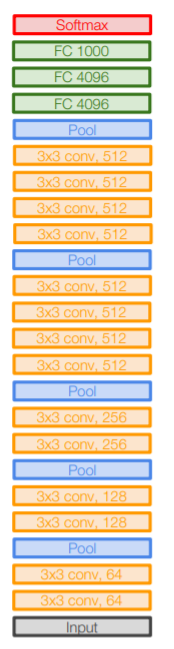
\includegraphics[scale=1.0]{images/Chapter4/vgg19_arch.png}
% \caption{VGG19 Model Architecture \cite{vgg19_architecture}}
% \label{vgg19_arch}
% \end{figure}
% \par
% VGG (Visual Geometry Group) was introduced by Simonyan Zisserman in 2014 at the University of Oxford. The difference between VGG16 and VGG19 is that they contain 16 and 19 layers respectively. VGG19 consists of 16 convolutional layers where each layer strictly used 3x3 filters with stride and a pad of size 1 and 3 fully connected layers, along with 2x2 max-pooling layers with stride 2. For simplicity and to lower down the parameters, it uses small 3x3 filters in convolutional layers. The fully connected layers contain 4,096 neurons followed by a softmax classifier. The network in VGG19 is simple but contain a lot of parameters and requires a lot of computational power. VGG19 is trained on the ImageNet database and can classify approximately more than 1000 object categories.